\documentclass[a4paper,12pt]{article}

\usepackage{mystyle}

\usepackage{gensymb}
\usepackage{scalerel}
\usepackage{stackengine}


\graphicspath{ {images/} }


% https://tex.stackexchange.com/questions/5461/is-it-possible-to-change-the-size-of-an-arrowhead-in-tikz-pgf
\usetikzlibrary{arrows.meta}


\DeclareMathOperator{\Image}{Im}

\definecolor{pink}{RGB}{218, 3, 174}
\definecolor{violet}{RGB}{148, 0, 211}
\definecolor{green}{RGB}{0, 153, 0}
\definecolor{orange}{RGB}{255, 153, 0}
\definecolor{blue}{RGB}{5, 73, 255}


% https://tex.stackexchange.com/a/101138/135045

\newcommand\widesim[1]{\ThisStyle{%
  \setbox0=\hbox{$\SavedStyle#1$}%
  \stackengine{-.1\LMpt}{$\SavedStyle#1$}{%
    \stretchto{\scaleto{\SavedStyle\mkern.2mu\sim}{.5150\wd0}}{.6\ht0}%
  }{O}{c}{F}{T}{S}%
}}


\newcommand{\BigMiddleThree}{\;\left|\vphantom{\begin{pmatrix} 0\\0\\0 \end{pmatrix}}\right.\;}
\newcommand{\BigMiddleFour}{\;\left|\vphantom{\begin{pmatrix} 0\\0\\0\\0 \end{pmatrix}}\right.\;}


% https://tex.stackexchange.com/questions/63531/how-to-write-quotation-marks-in-math-environment
\DeclareMathSymbol{\mlq}{\mathord}{operators}{``}
\DeclareMathSymbol{\mrq}{\mathord}{operators}{`'}


\DeclareMathOperator{\Imag}{Im}


% https://tex.stackexchange.com/questions/544453/undefined-control-sequence-after-paragraph
\renewcommand{\paragraph}[1]{\noindent\textbf{#1}\quad}


% https://tex.stackexchange.com/questions/36851/skipping-line-after-proof-in-proof-environment#comment73553_36851
\newcommand{\proofindent}{\hspace*{\fill}\par\vspace{0.5em}\noindent}


% https://tex.stackexchange.com/questions/4813/extendible-equals-sign
\makeatletter
\newcommand*{\Relbarfill@}{\arrowfill@\Relbar\Relbar\Relbar}
\newcommand*{\xeq}[2][]{\ext@arrow 0055\Relbarfill@{#1}{#2}}
\makeatother


% https://tex.stackexchange.com/questions/279100/typeset-the-shrug-%C2%AF-%E3%83%84-%C2%AF-emoji
\newcommand{\shrug}[1][]{%
\begin{tikzpicture}[baseline,x=0.8\ht\strutbox,y=0.8\ht\strutbox,line width=0.125ex,#1]
  \def\arm{(-2.5,0.95) to (-2,0.95) (-1.9,1) to (-1.5,0) (-1.35,0) to (-0.8,0)};
  \draw \arm;
  \draw[xscale=-1] \arm;
  \def\headpart{(0.6,0) arc[start angle=-40, end angle=40,x radius=0.6,y radius=0.8]};
  \draw \headpart;
  \draw[xscale=-1] \headpart;
  \def\eye{(-0.075,0.15) .. controls (0.02,0) .. (0.075,-0.15)};
  \draw[shift={(-0.3,0.8)}] \eye;
  \draw[shift={(0,0.85)}] \eye;
  % draw mouth
  \draw (-0.1,0.2) to [out=15,in=-100] (0.4,0.95); 
\end{tikzpicture}}


% TODO: package installation failed for some reason, so I had to use good old copy-paste...
%
% Here are some links to make the copy-paste look more decent.
%
% The Comprehensive LaTeX Symbol List (page 143):
% * https://tug.ctan.org/info/symbols/comprehensive/symbols-a4.pdf
%
% utfsym package (file source/usym2740.tikz):
% * https://ctan.org/pkg/utfsym
% * https://gitlab.com/gi-fg-ibnw/utfsym/-/tree/master
\newcommand{\usym}{\resizebox{!}{\fontcharht\font`M}{
  \begin{tikzpicture}[y=0.80pt, x=0.80pt, yscale=-1.000000, xscale=1.000000, inner sep=0pt, outer sep=0pt]
  \begin{scope}[shift={(100.0,1831.0)},nonzero rule]
    \path[draw=.,fill=.,line width=1.600pt] (1626.0000,-813.0000) ..
      controls (1626.0000,-730.3333) and (1600.0000,-664.3333) ..
      (1548.0000,-615.0000) .. controls (1496.6667,-566.3333) and
      (1431.3333,-542.0000) .. (1352.0000,-542.0000) .. controls
      (1342.6667,-542.0000) and (1333.0000,-542.3333) .. (1323.0000,-543.0000) --
      (1177.0000,-555.0000) .. controls (1359.0000,-456.3333) and
      (1450.0000,-348.3333) .. (1450.0000,-231.0000) .. controls
      (1450.0000,-163.0000) and (1423.0000,-102.6667) .. (1369.0000,-50.0000) ..
      controls (1315.6667,2.6667) and (1255.0000,29.0000) .. (1187.0000,29.0000) ..
      controls (1013.6667,29.0000) and (908.0000,-96.6667) .. (870.0000,-348.0000)
      .. controls (858.0000,-286.6667) and (849.0000,-245.3333) ..
      (843.0000,-224.0000) .. controls (829.6667,-177.3333) and (812.6667,-138.0000)
      .. (792.0000,-106.0000) .. controls (734.6667,-16.0000) and (659.0000,29.0000)
      .. (565.0000,29.0000) .. controls (491.0000,29.0000) and (427.0000,2.6667) ..
      (373.0000,-50.0000) .. controls (319.6667,-103.3333) and (293.0000,-166.6667)
      .. (293.0000,-240.0000) .. controls (293.0000,-312.0000) and
      (319.6667,-375.0000) .. (373.0000,-429.0000) .. controls (407.0000,-463.6667)
      and (465.6667,-504.3333) .. (549.0000,-551.0000) -- (432.0000,-545.0000) ..
      controls (343.3333,-540.3333) and (267.6667,-560.6667) .. (205.0000,-606.0000)
      .. controls (135.0000,-656.0000) and (100.0000,-725.0000) ..
      (100.0000,-813.0000) .. controls (100.0000,-889.0000) and (125.0000,-952.6667)
      .. (175.0000,-1004.0000) .. controls (225.6667,-1055.3333) and
      (289.3333,-1081.0000) .. (366.0000,-1081.0000) .. controls
      (457.3333,-1081.0000) and (559.0000,-1025.0000) .. (671.0000,-913.0000) ..
      controls (622.3333,-1033.0000) and (598.0000,-1122.0000) ..
      (598.0000,-1180.0000) .. controls (598.0000,-1256.0000) and
      (621.6667,-1319.0000) .. (669.0000,-1369.0000) .. controls
      (716.3333,-1419.0000) and (777.3333,-1444.0000) .. (852.0000,-1444.0000) ..
      controls (927.3333,-1444.0000) and (991.3333,-1420.0000) ..
      (1044.0000,-1372.0000) .. controls (1098.6667,-1322.0000) and
      (1126.0000,-1260.0000) .. (1126.0000,-1186.0000) .. controls
      (1126.0000,-1120.0000) and (1100.6667,-1032.6667) .. (1050.0000,-924.0000) ..
      controls (1167.3333,-1028.6667) and (1274.0000,-1081.0000) ..
      (1370.0000,-1081.0000) .. controls (1440.6667,-1081.0000) and
      (1501.0000,-1054.3333) .. (1551.0000,-1001.0000) .. controls
      (1601.0000,-947.6667) and (1626.0000,-885.0000) .. (1626.0000,-813.0000) --
      cycle(1505.0000,-805.0000) .. controls (1505.0000,-861.6667) and
      (1485.3333,-908.0000) .. (1446.0000,-944.0000) .. controls
      (1408.0000,-978.0000) and (1360.6667,-995.0000) .. (1304.0000,-995.0000) ..
      controls (1182.0000,-995.0000) and (1090.6667,-941.3333) ..
      (1030.0000,-834.0000) -- (1081.0000,-772.0000) -- (1245.0000,-811.0000) ..
      controls (1283.0000,-820.3333) and (1302.0000,-816.3333) ..
      (1302.0000,-799.0000) .. controls (1302.0000,-787.6667) and
      (1287.0000,-775.3333) .. (1257.0000,-762.0000) -- (1106.0000,-694.0000) --
      (1106.0000,-612.0000) .. controls (1158.6667,-600.0000) and
      (1203.6667,-594.0000) .. (1241.0000,-594.0000) .. controls
      (1311.0000,-594.0000) and (1371.0000,-611.3333) .. (1421.0000,-646.0000) ..
      controls (1477.0000,-684.6667) and (1505.0000,-737.6667) ..
      (1505.0000,-805.0000) -- cycle(1054.0000,-1087.0000) .. controls
      (1054.0000,-1153.6667) and (1038.0000,-1208.3333) .. (1006.0000,-1251.0000) ..
      controls (970.0000,-1297.6667) and (920.0000,-1321.0000) ..
      (856.0000,-1321.0000) .. controls (792.6667,-1321.0000) and
      (744.0000,-1296.0000) .. (710.0000,-1246.0000) .. controls
      (680.0000,-1202.0000) and (665.0000,-1147.0000) .. (665.0000,-1081.0000) ..
      controls (665.0000,-1008.3333) and (691.6667,-938.6667) ..
      (745.0000,-872.0000) -- (821.0000,-899.0000) -- (835.0000,-1069.0000) ..
      controls (837.6667,-1103.0000) and (845.3333,-1120.0000) ..
      (858.0000,-1120.0000) .. controls (865.3333,-1120.0000) and
      (873.3333,-1103.0000) .. (882.0000,-1069.0000) -- (909.0000,-899.0000) --
      (974.0000,-872.0000) .. controls (1027.3333,-945.3333) and
      (1054.0000,-1017.0000) .. (1054.0000,-1087.0000) -- cycle(1341.0000,-276.0000)
      .. controls (1341.0000,-340.6667) and (1313.6667,-399.0000) ..
      (1259.0000,-451.0000) .. controls (1210.3333,-498.3333) and
      (1152.3333,-530.3333) .. (1085.0000,-547.0000) -- (1044.0000,-489.0000) --
      (1134.0000,-346.0000) .. controls (1149.3333,-327.3333) and
      (1157.0000,-311.6667) .. (1157.0000,-299.0000) .. controls
      (1157.0000,-288.3333) and (1151.3333,-283.0000) .. (1140.0000,-283.0000) ..
      controls (1132.6667,-283.0000) and (1117.6667,-294.3333) ..
      (1095.0000,-317.0000) -- (977.0000,-436.0000) -- (909.0000,-412.0000) ..
      controls (907.6667,-401.3333) and (907.0000,-390.3333) .. (907.0000,-379.0000)
      .. controls (907.0000,-306.3333) and (930.3333,-240.6667) ..
      (977.0000,-182.0000) .. controls (1026.3333,-119.3333) and
      (1086.3333,-88.0000) .. (1157.0000,-88.0000) .. controls (1207.0000,-88.0000)
      and (1250.0000,-107.0000) .. (1286.0000,-145.0000) .. controls
      (1322.6667,-183.0000) and (1341.0000,-226.6667) .. (1341.0000,-276.0000) --
      cycle(690.0000,-831.0000) .. controls (618.0000,-937.6667) and
      (527.6667,-991.0000) .. (419.0000,-991.0000) .. controls (365.0000,-991.0000)
      and (318.6667,-972.6667) .. (280.0000,-936.0000) .. controls
      (242.0000,-899.3333) and (223.0000,-854.3333) .. (223.0000,-801.0000) ..
      controls (223.0000,-736.3333) and (252.3333,-683.0000) .. (311.0000,-641.0000)
      .. controls (364.3333,-603.0000) and (425.0000,-584.0000) ..
      (493.0000,-584.0000) .. controls (519.6667,-584.0000) and (563.3333,-592.6667)
      .. (624.0000,-610.0000) -- (624.0000,-692.0000) -- (471.0000,-756.0000) ..
      controls (436.3333,-766.0000) and (419.0000,-778.3333) .. (419.0000,-793.0000)
      .. controls (419.0000,-807.0000) and (439.0000,-810.3333) ..
      (479.0000,-803.0000) -- (645.0000,-772.0000) -- (690.0000,-831.0000) --
      cycle(831.0000,-412.0000) -- (757.0000,-436.0000) -- (641.0000,-309.0000) ..
      controls (627.0000,-290.3333) and (615.3333,-281.0000) .. (606.0000,-281.0000)
      .. controls (596.6667,-281.0000) and (592.0000,-285.6667) ..
      (592.0000,-295.0000) .. controls (592.0000,-304.3333) and (597.3333,-318.6667)
      .. (608.0000,-338.0000) -- (692.0000,-489.0000) -- (645.0000,-549.0000) ..
      controls (483.6667,-491.6667) and (403.0000,-399.3333) .. (403.0000,-272.0000)
      .. controls (403.0000,-223.3333) and (421.6667,-180.3333) ..
      (459.0000,-143.0000) .. controls (497.0000,-106.3333) and (540.3333,-88.0000)
      .. (589.0000,-88.0000) .. controls (657.6667,-88.0000) and
      (716.3333,-119.3333) .. (765.0000,-182.0000) .. controls (811.0000,-240.6667)
      and (834.0000,-305.3333) .. (834.0000,-376.0000) .. controls
      (834.0000,-388.6667) and (833.0000,-400.6667) .. (831.0000,-412.0000) --
      cycle;
  \end{scope}
  \end{tikzpicture}
}}


\theoremstyle{remark}
\newtheorem*{finalsolution}{Решение}
\AtEndEnvironment{finalsolution}{\hfill\usym}



\author{Алексеев Василий}


\title{Семинар 11}
\date{21 + 25 апреля 2023}


\begin{document}
  \maketitle
  
  \tableofcontents

  \thispagestyle{empty}
  
  \newpage
  
  
  
  \vspace*{\fill}
  
  \noindent
  \emph{
    Жирным шрифтом обозначаются как векторы линейного пространства, так и их координатные столбцы в выбранном базисе.
    При этом и векторы, и их координатные столбцы обозначаются, как правило, одинаковыми буквами.
    Например, $\bds x \hm\in X$ (вектор) и $\bds x \hm\in \RR^{\dim X}$ (его координатный столбец).
    Таким образом, смысл зависит от контекста
  } \shrug
  
  \vspace*{\fill}
  
  \thispagestyle{empty}
  
  \newpage
  
  
  \pagenumbering{arabic}


  \section{Adjo \& Ortho (Diag E1)}
  
  \subsection{Самосопряжённые преобразования}
  
  \subsubsection{Собственные + ортогонализация, или \# 29.19(7)}\label{p29-19}
  
  Преобразование $\phi\hm\colon \mathcal E \hm\to \mathcal E$, где $\mathcal E$~---~евклидово пространство, задано в некотором \emph{ортонормированном базисе}~$e \hm= (\bds e_1, \bds e_2, \bds e_3)$ матрицей:
  \[
    A = \begin{pmatrix}
      1 & -4 & 1\\
      -4 & 16 & -4\\
      1 & -4 & 1
    \end{pmatrix}
  \]
  Надо найти \emph{ортонормированный базис из собственных векторов} преобразования~$\phi$, матрицу перехода~$S$ к этому базису, и матрицу~$A'$ преобразования~$\phi$ в этом базисе.
  
  \begin{solution}
  
  Найдём \textbf{собственные значения} преобразования $\phi$.
  Характеристическое уравнение:
  \[
    \det (A - \lambda E) = 0
  \]
  \[
    \begin{vmatrix}
      1 - \lambda & -4 & 1\\
      -4 & 16 - \lambda & -4\\
      1 & -4 & 1 - \lambda
    \end{vmatrix} = \ldots = \lambda^2 (18 - \lambda) = 0
    \Rightarrow \left[
      \begin{aligned}
        &\lambda = 0\quad \mbox{(кратность $2$)}\\
        &\lambda = 18
      \end{aligned}
    \right.
  \]
  
  Видно, что \emph{все корни характеристического уравнения вещественные}, поэтому они же~---~и собственные значения преобразования $\phi$.
  
  При этом то, что $\lambda \hm= 0$~---~собственное значение, можно бы было заметить и в самом начале, ведь у матрицы $A$ строки уже линейно зависимы (первая и третья совпадают), то есть $\det(A \hm- \lambda E)|_{\lambda = 0} \hm= 0$.
  
  \medskip
  
  Найдём \textbf{собственные векторы} преобразования $\phi$ (максимальную линейно независимую систему собственных векторов).
  При $\lambda \hm= 0$ получаем следующее уравнение для поиска собственных векторов:
  \[
    A \bds x = \lambda \bds x
  \]
  \[
    (A - \lambda E) \bds x = \bds 0
  \]
  \[
    \begin{pmatrix}
      1 & -4 & 1\\
      -4 & 16 & -4\\
      1 & -4 & 1
    \end{pmatrix} \begin{pmatrix}
      x_1 \\ x_2 \\ x_3
    \end{pmatrix} = \bds 0
  \]
  
  Последнее матричное уравнение равносильно одному скалярному уравнению
  \[
    x_1 - 4 x_2 + x_3 = 0
  \]
  
  Из которого можно, например, выразить $x_1$ через $x_2$ и $x_3$:
  \[
    x_1 = 4 t_1 - t_2,\quad x_2 = t_1 \in \RR,\quad x_3 = t_2 \in \RR
  \]
  
  Тогда общее решение $A \bds x \hm= \bds 0$ (произвольный вектор из собственного подпространства $\Ker (A \hm- \lambda E)|_{\lambda = 0}$) можно выписать в виде:
  \[
    \bds x = \begin{pmatrix}
      4 t_1 - t_2\\
      \hphantom{4} t_1 \hphantom{- t_2}\\
      \hphantom{4 t_1 -} t_2
    \end{pmatrix}
    = t_1 \cdot \begin{pmatrix}
      4 \\ 1 \\ 0
    \end{pmatrix}
    + t_2 \cdot \begin{pmatrix}
      -1 \\ 0 \\ 1
    \end{pmatrix}
  \]
  
  Видно, что в качестве базиса в собственном подпространстве $\phi$, соответствующем собственному значению $\lambda \hm= 0$ (максимальная линейно независимая система собственных векторов для $\lambda \hm= 0$) можно взять векторы:
  \[
    \bds x_1 = \begin{pmatrix}
      4 \\ 1 \\ 0
    \end{pmatrix},\quad
    \bds x_2 = \begin{pmatrix}
      -1 \\ 0 \\ 1
    \end{pmatrix}
  \]
  
  (Не лишним будет на всякий случай убедиться, что в самом деле $A \bds x_1 \hm= \bds 0$ и $A \bds x_2 \hm= \bds 0$.)
  
  \medskip
  
  Теперь найдём собственные векторы для $\lambda \hm= 18$.
  Уравнение, определяющее соответствующее собственное подпространство:
  \[
    \begin{pmatrix}
      -17 & -4 & 1\\
      -4 & -2 & -4\\
      1 & -4 & -17
    \end{pmatrix} \begin{pmatrix}
      x_1 \\ x_2 \\ x_3
    \end{pmatrix} = \bds 0
  \]
  
  Упростим матрицу полученной однородной системы:
  \[
    \begin{pmatrix}
      -17 & -4 & 1\\
      -4 & -2 & -4\\
      \bds{1} & -4 & -17
    \end{pmatrix}
    \sim \begin{pmatrix}
      0 & -72 & -288\\
      0 & -18 & -72\\
      1 & -4 & -17
    \end{pmatrix}
    \sim \begin{pmatrix}
      0 & 1 & 4\\
      0 & \bds{1} & 4\\
      1 & -4 & -17
    \end{pmatrix}
    \sim \begin{pmatrix}
      0 & 0 & 0\\
      0 & 1 & 4\\
      1 & 0 & -1
    \end{pmatrix}
  \]
  
  Упрощённая система будет выглядеть следующим образом:
  \[
    \left\{
      \begin{aligned}
        &\hphantom{x_1 +} x_2 + 4 x_3 = 0\\
        &x_1 \hphantom{+ x_2} - \hphantom{4} x_3 = 0
      \end{aligned}
    \right.
    \quad\leftrightarrow\quad \left\{
      \begin{aligned}
        &x_2 = -4 x_3\\
        &x_1 = x_3
      \end{aligned}
    \right.
  \]
  
  Общее решение:
  \[
    \bds x = \begin{pmatrix}
      t \\ -4t \\ t
    \end{pmatrix}
    = t \cdot \begin{pmatrix}
      1 \\ -4 \\ 1
    \end{pmatrix},\quad t \in \RR
  \]
  
  Базис в собственном подпространстве (один вектор):
  \[
    \bds x_3 = \begin{pmatrix}
      1 \\ -4 \\ 1
    \end{pmatrix}
  \]
  
  (На всякий случай убеждаемся, что $A \bds x_3 = 18 \bds x_3$.)
  
  \medskip
  
  Таким образом, мы нашли \emph{базис из собственных векторов} преобразования $\phi$:
  \begin{equation}\label{p29-19:basis}
    \{\bds x_1, \bds x_2, \bds x_3\} = \left\{
      \begin{pmatrix}
        4 \\ 1 \\ 0
      \end{pmatrix},
      \begin{pmatrix}
        -1 \\ 0 \\ 1
      \end{pmatrix},
      \begin{pmatrix}
        1 \\ -4 \\ 1
      \end{pmatrix}
    \right\}
  \end{equation}
  
  \medskip
  
  Теперь проведём \textbf{ортогонализацию} системы векторов (\ref{p29-19:basis}).
  Исходный базис~$e$ ортонормированный, поэтому скалярное произведение между векторами $\bds x \hm= (x_1, \ldots, x_n)^T$ и $\bds y \hm= (y_1, \ldots, y_n)^T$ считается ``по-простому''\footnote{Кстати, похоже, что в англоязычных источниках ``скалярным произведением'' называется именно эта \href{https://en.wikipedia.org/wiki/Dot_product\#Coordinate\_definition}{``простая формула'' скалярного произведения}: сумма произведений соответствующих координат. Именуется как \emph{dot product} или \emph{scalar product}. Термином же \emph{inner product} обозначается \href{https://en.wikipedia.org/wiki/Inner\_product\_space}{скалярное произведение вообще}. То есть, \href{https://math.stackexchange.com/a/476742/451127}{ещё раз}: наше ``скалярное произведение''~---~их ``inner product'', наше ``скалярное произведение в ортонормированном базисе''~---~их ``dot product'' или ``scalar product''. Something like this... Looks like... Anyway.}:
  \[
    (\bds x, \bds y) = x_1 y_1 + \ldots + x_n y_n
  \]
  
  Видно, что $(\bds x_1, \bds x_3) \hm= 4 \hm- 4 \hm+ 0 \hm= 0$.
  Так же, как и $(\bds x_2, \bds x_3) \hm= -1 \hm+ 0 \hm+ 1 \hm= 0$.
  То есть \emph{собственные векторы, соответствующие различным собственным значениям преобразования~$\phi$, ортогональны}.
  
  Остаётся ``поправить'' подсистему $\{\bds x_1, \bds x_2\}$, потому что $(\bds x_1, \bds x_2) \hm= -4 \hm{\not=} 0$.
  Вычтем, например, из $\bds x_1$ его ортогональную проекцию на $\bds x_2$:
  \[
    \bds x_1' \equiv \bds x_1 - \frac{(\bds x_1, \bds x_2)}{|\bds x_2|} \cdot \frac{\bds x_2}{|\bds x_2|}
    = \begin{pmatrix}4 \\ 1 \\ 0\end{pmatrix} + 2 \begin{pmatrix}-1 \\ 0 \\ 1\end{pmatrix}
    = \begin{pmatrix}2 \\ 1 \\ 2\end{pmatrix}
  \]
  где было использовано, что $|\bds x_2|^2 \hm= 1 \hm+ 0 \hm+ 1 \hm= 2$.
  
  Убеждаемся, что $(\bds x_1', \bds x_2) \hm= -2 \hm+ 0 \hm+ 2 \hm= 0$.
  Так как мы считали $\bds x_1'$ как линейную комбинацию $\bds x_1$ и $\bds x_2$, то должно получиться $(\bds x_1', \bds x_3) \hm= 0$ (то есть можно не проверять ортогональность с $\bds x_3$; ну, или можно проверить, но стоит понимать, что ничего удивительного в сохранении ортогональности $\bds x_1'$ и $\bds x_3$ нет).
  Получили ортогональную систему $\{\bds x_1', \bds x_2, \bds x_3\}$ из собственных векторов преобразования $\phi$?..
  А остался ли вектор $\bds x_1'$ собственным для $\lambda \hm= 0$?
  Да, ведь он получен как линейная комбинация $\bds x_1$ и $\bds x_2$~---~векторов из собственного подпространства $\Ker(A \hm- \lambda E)|_{\lambda = 0}$, а потому $\bds x_1'$ тоже лежит в указанном собственном подпространстве:
  \[
    \phi(\bds x_1') = \phi(\bds x_1 + 2 \bds x_2) = \phi(\bds x_1) + \phi(2 \bds x_2) = \ldots = \lambda (\bds x_1 + 2 \bds x_2) = \lambda \bds x_1'
  \]
  
  Итого, помимо просто базиса из собственных векторов, для преобразования~$\phi$ \emph{существует ортогональный базис из собственных векторов} (ради однообразия обозначений положим $\bds x_2' \hm\equiv \bds x_2$, $\bds x_3' \hm\equiv \bds x_3$):
  \begin{equation}\label{p29-19:orto-basis}
    \{\bds x_1', \bds x_2', \bds x_3'\} = \left\{
      \begin{pmatrix}
        2 \\ 1 \\ 2
      \end{pmatrix},
      \begin{pmatrix}
        -1 \\ 0 \\ 1
      \end{pmatrix},
      \begin{pmatrix}
        1 \\ -4 \\ 1
      \end{pmatrix}
    \right\}
  \end{equation}
  
  \medskip
  
  Можно ещё \textbf{нормировать} базис~---~поделив все векторы (\ref{p29-19:orto-basis}) на их модули:
  \[
    \left\{
      \begin{aligned}
        &|\bds x_1'| = \sqrt{4 + 1 + 4} = 3\\
        &|\bds x_2'| = \sqrt{1 + 1} = \sqrt{2}\\
        &|\bds x_3'| = \sqrt{1 + 16 + 1} = 3 \sqrt{2}
      \end{aligned}
    \right.
  \]
  
  Получим следующий \emph{ортонормированный базис из собственных векторов}:
  \begin{equation}\label{p29-19:ortonorm-basis}
    \{\bds x_1'', \bds x_2'', \bds x_3''\} = \left\{
      \frac{1}{3} \begin{pmatrix}
        2 \\ 1 \\ 2
      \end{pmatrix},
      \frac{1}{\sqrt{2}} \begin{pmatrix}
        -1 \\ 0 \\ 1
      \end{pmatrix},
      \frac{1}{3 \sqrt{2}} \begin{pmatrix}
        1 \\ -4 \\ 1
      \end{pmatrix}
    \right\}
  \end{equation}
  
  \medskip
  
  Матрица перехода $S$ от старого ортонормированного базиса~$e$ в новому $\{\bds x_1'', \bds x_2'', \bds x_3''\}$~---~это матрица, столбцы которой есть компоненты новых базисных векторов в старом базисе.
  То есть матрица $S$ получается просто объединением столбцов (\ref{p29-19:ortonorm-basis}) в матрицу:
  \[
    S = \begin{pmatrix}
      2 / 3 & -1 / \sqrt{2} & 1 / \left(3 \sqrt{2}\right)\\
      1 / 3 & 0             & -4 / \left(3 \sqrt{2}\right)\\
      2 / 3 & 1 / \sqrt{2}  & 1 / \left(3 \sqrt{2}\right)
    \end{pmatrix}
  \]
  
  Можно заметить, что $S^T S \hm= E$, то есть матрица перехода $S$ ортогональная.
  Это потому, что $S$~---~матрица перехода от \emph{одного ортонормированного} базиса к \emph{другому ортонормированному} базису.
  Например, чему равен элемент в матрице $S^T S$ в первой строчке и втором столбце:
  \[
    (S^T S)_{12} = \bds x_1''^T \bds x_2'' \xeq{\mbox{\footnotesize старый ОНБ}} (\bds x_1'', \bds x_2'') \xeq{\mbox{\footnotesize новый ОНБ}} 0
  \]
  
  \medskip
  
  Чтобы найти матрицу $A'$ преобразования $\phi$ в новом базисе, можно воспользоваться либо тем, что новый базис~---~это базис из собственных векторов (например, в новом базисе $\bds x_1''$ имеет координаты $(1, 0, 0)^T$, поэтому образ $\bds x_1''$ будет просто первым столбцом $A'$, а это $\lambda \bds x_1''|_{\lambda = 0}$, так как вектор $\bds x_1''$~---~собственный, соответствующий $\lambda \hm= 0$), то есть
  \[
    A' = \begin{pmatrix}
      0 & 0 & 0\\
      0 & 0 & 0\\
      0 & 0 & 18
    \end{pmatrix}
  \]
  
  Либо тем, что уже известна матрица $S$ перехода от старого базиса к новому:
  \[
    A' = S^{-1} A S \xeq{S^T S = E} S^T A S = \ldots = \begin{pmatrix}
      0 & 0 & 0\\
      0 & 0 & 0\\
      0 & 0 & 18
    \end{pmatrix}
  \]
  
  Первый способ, очевидно, побыстрее :)
  Но вторым, с матрицей $S$, можно хотя бы проверить, что всё в порядке.
  Если только не ошибиться в процессе самой проверки :)
  \end{solution}
  
  
  
  \subsubsection{Кусочек теории, или Попытка принять}
  
  Пусть есть линейное преобразование $\phi\hm\colon \mathcal E \hm\to \mathcal E$ \emph{евклидова} пространства $\mathcal E$ (то есть пространство, в котором \emph{выбрано} скалярное произведение $(\cdot, \cdot)$).
  Тогда преобразованием, \emph{сопряжённым} преобразованию $\phi$, называется преобразование $\phi^*\hm\colon \mathcal E \hm\to \mathcal E$, такое что
  \begin{equation}\label{eq:adjoint}
    \boxed{\bigl(\phi(\bds x), \bds y\bigr) = \bigl(\bds x, \phi^*(\bds y)\bigr),\quad \forall \bds x, \bds y \in \mathcal E}
  \end{equation}
  
  Существует ли вообще для данного~$\phi$ сопряжённое ему~$\phi^*$?
  Пусть $e$~---~базис в $\mathcal E$.
  Пусть матрица $\Gamma$~---~матрица Грама базиса~$e$, $A$~---~матрица преобразования $\phi$ в базисе~$e$, и $A^*$~---~матрица сопряжённого преобразования~$\phi^*$ (предполагаем, что оно существует).
  Тогда левую часть соотношения (\ref{eq:adjoint}) можно переписать в таком виде:
  \[
    (\phi(\bds x), \bds y) = (A \bds x)^T \Gamma \bds y = \bds x^T \cdot A^T \Gamma \cdot \bds y
  \]
  
  А правая часть (\ref{eq:adjoint}) будет выглядеть как
  \[
    (\bds x, \phi^*(\bds y)) = \bds x^T \Gamma (A^* \bds y) = \bds x^T \cdot \Gamma A^* \cdot \bds y
  \]
  
  Так как (\ref{eq:adjoint}) верно для произвольной пары $(\bds x, \bds y)$, то равны ``матрицы посередине'':
  \begin{equation}
    \boxed{A^T \Gamma = \Gamma A^*}
  \end{equation}
  
  Так как $\Gamma$~---~матрица Грама (обязательно $\det \Gamma \hm{\not=} 0$), то можно соотношение между матрицами исходного и сопряжённого преобразований переписать в таком виде:
  \[
    A^* = \Gamma^{-1} A^T \Gamma
  \]
  
  Получается, \emph{для произвольного преобразования~$\phi$ евклидова пространства существует, причём единственное, сопряжённое преобразование~$\phi^*$}.
  
  Матрица сопряжённого преобразования в \emph{ортонормированном базисе}:
  \[
    A^* = A^T\quad \mbox{(ОНБ)}
  \]
  
  \medskip
  
  Преобразование $\phi$ евклидова пространства $\mathcal E$ называется \emph{самосопряжённым}, если оно совпадает со своим сопряжённым $\phi^*$, то есть $\phi(\bds x) \hm= \phi^*(\bds x)$, $\forall \bds x \hm\in \mathcal E$, или:
  \begin{equation}\label{eq:self-adjoint-def}
    \boxed{
      \bigl(\phi(\bds x), \bds y\bigr) = \bigl(\bds x, \phi(\bds y)\bigr),\quad \forall \bds x, \bds y \in \mathcal E
    }
  \end{equation}
  
  Матрица~$A$ самосопряжённого преобразования удовлетворяет соотношению:
  \begin{equation}\label{eq:self-adjoint}
    A^T \Gamma = \Gamma A
  \end{equation}
  
  В ортонормированном базисе:
  \begin{equation}\label{eq:self-adjoint-onb}
    \boxed{A = A^T\quad \mbox{(ОНБ)}}
  \end{equation}
  
  \begin{proposition}[``Матричный критерий самосопряжённости'']
    Если преобразование самосопряжённое, то его матрица в любом ортонормированном базисе симметричная.
    Обратно, если в некотором ортонормированном базисе матрица преобразования симметричная, то оно обязательно самосопряжённое.
  \end{proposition}
  
  \medskip
  
  Оказывается, что с самосопряжёнными преобразованиями связано несколько ``интересных'' утверждений в контексте собственных значений и собственных векторов...
  
  \begin{theorem}\label{theo:real-roots}
    Все корни характеристического уравнения самосопряжённого преобразования вещественные\footnote{При этом интересно, что корни характеристического уравнения~---~это характеристика именно преобразования, а свойство самосопряжённости связано с выбором скалярного произведения...}.
  \end{theorem}
  
  \begin{example}
    Убедимся в этом на примере самосопряжённого преобразования двумерного пространства, заданного матрицей в ортонормированном базисе (симметричной).
    Пусть матрица преобразования $A \hm= \left(\begin{smallmatrix}a & b\\ b & c\end{smallmatrix}\right)$.
    Тогда характеристическое уравнение:
    \[
      \det(A - \lambda E) = \begin{vmatrix}
        a - \lambda & b\\
        b & c - \lambda
      \end{vmatrix} = 0
    \]
    \[
      \lambda^2 - (a + c) \lambda + (b^2 + ac) = 0
    \]
    
    Дискриминант $(a \hm+ c)^2 \hm- 4(b^2 \hm+ ac) \hm= (a \hm- c)^2 \hm+ b^2 \hm\geq 0$, поэтому оба корня $\lambda_{1, 2} \hm\in \RR$.
  \end{example}
  
  Хорошо, с самосопряжённым преобразованием двумерного пространства понятно.
  А что же в случае $n$-мерного пространства?
  Как быть там?
  Логика-то для двумерного на $n$-мерное как-то ``не очень'' распространяется...
  

  \newpage
  
  \noindent
  \textbf{``Попытка принять''}\footnote{На основе \href{https://joisino.net/2021/03/18/spectral}{joisino.net/2021/03/18/spectral}.}

  Пусть есть самосопряжённое преобразование~$\phi$ с матрицей~$A$ (в выбранном базисе пространства~$\mathcal E$).
  ``Посмотрим'' на него внимательнее.
  
  Для некоторых (произвольно выбранных) векторов $\bds x$ и $\bds y$ выполнено:
  \begin{equation}\label{eq:x-dot-Ax-Ax-dot-y}
    (\bds x, A \bds y) = (A \bds x, \bds y)
  \end{equation}
  Будем считать, что $|\bds x| \hm= |\bds y| \hm= 1$ (для определённости рассматриваем только нормированные векторы).
  Заметим, что при фиксированном~$\bds x$ скалярное произведение $(A \bds x, \bds y)$ достигает максимума, очевидно, при $\bds y \hm\upuparrows A \bds x$.
  Но в силу сопряжённости преобразования $\phi$ имеем соотношение~(\ref{eq:x-dot-Ax-Ax-dot-y}).
  Таким образом:
  \begin{equation}\label{eq:min-max-scalar}
    \left\{
      \begin{aligned}
        &\max_{|\bds y| = 1} (\bds x, A \bds y) \Leftrightarrow \bds y \upuparrows A \bds x\\
        &\min_{|\bds y| = 1} (\bds x, A \bds y) \Leftrightarrow \bds y \updownarrows A \bds x
      \end{aligned}
    \right.
  \end{equation}
  то есть при любом $\bds x$, $|\bds x| \hm= 1$ существует и единствен вектор $\bds y$, $|\bds y| \hm= 1$, на котором достигает максимум функция от $\bds y$ вида $(\bds x, A \bds y)$ (кроме случая, когда $A \bds x \hm= \bds 0$~---~тогда при любом $\bds y$ будет получаться ноль): это вектор~$\bds y \hm\upuparrows A \bds x$~(\ref{fig:self-adjo-on-the-way-to-understand}).
  
  \begin{figure}
    \centering
    
    
\includegraphics[width=0.5\columnwidth]{self-adjo-on-the-way-to-understand}
    
    \caption{Из самосопряжённости преобразования с матрицей~$A$ следует, что при фиксированном векторе~$\bds x$ из всех векторов $\bds y$ единичной длины $|\bds y| \hm= 1$ именно при $\bds y \hm\upuparrows A \bds x$ максимально скалярное произведение $(\bds x, A \bds y)$. Но будет ли при этом вектор $A \bds y$ параллелен вектору~$\bds x$?..}
    \label{fig:self-adjo-on-the-way-to-understand}
  \end{figure}
  
  Будет ли вектор $A \bds y$ параллелен $\bds x$?
  Нет, гарантировать такого нельзя.
  (Пока нельзя?)
  \emph{А что, если окажется $A \bds y \hm\parallel \bds x$}?
  Тогда получится, что под действием $\phi$ вектор $\bds x$ переходит в $A \bds x$, который, в свою очередь, в результате применения к нему~$\phi$ снова пойдёт по направлению вектора~$\bds x$.
  То есть как бы переход ``туда-обратно''.
  И вследствие линейности преобразования~$\phi$ \emph{можно предположить, что ``посередине'' между $\bds x$ и $A \bds x$ окажется вектор~$\bds z$, который не ходит ``туда-сюда'' при действии~$\phi$, а ``стоит на месте'', то есть его образ~$A \bds z$ не ``отклоняется'' от исходного~$\bds z$, а остаётся ему параллелен: $A \bds z \hm\parallel \bds z$~---~этот вектор~$\bds z$ и будет собственным}~(\ref{fig:self-adjo-eigen-here-you-are})!
  
  \begin{figure}
    \centering
    
    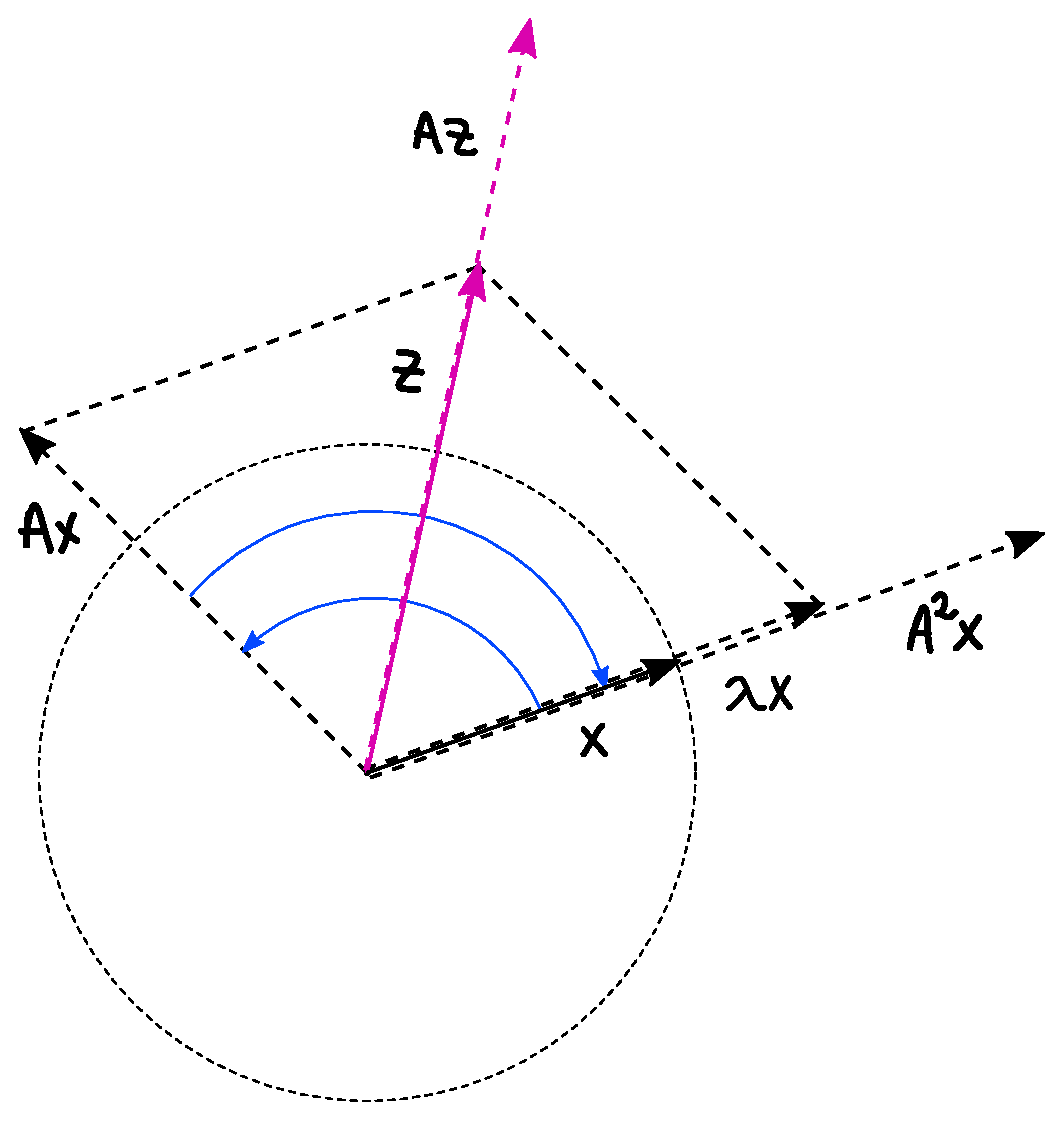
\includegraphics[width=0.56\columnwidth]{self-adjo-eigen-here-you-are}
    
    \caption{Если после действия~$\phi$ вектор~$A \bds x$ станет параллелен исходному вектору~$\bds x$, то можно ожидать, что ``посередине'' найдётся собственный вектор~$\bds z$ (который в результате действия~$\phi$ вообще ``не отклоняется'' от первоначального направления). Посередине~---~значит, его можно выразить как $\bds z \hm= A \bds x \hm+ \lambda \bds x$, где $\lambda \hm= |A \bds x|$.}
    \label{fig:self-adjo-eigen-here-you-are}
  \end{figure}
  
  % Maybe that's interesting, in some way, but I do not think it helps in understanding the topic...
  %
  %А что, если бы мы хотели максимизировать функцию вида $(\bds x, A \bds x)$, $|\bds x| \hm= 1$?
  %По рассмотренному ранее, кажется, что решение должно быть таким:
  %\[
    %\max_{|\bds x| = 1} (\bds x, A \bds x) \Leftarrow \underline{\bds x \upuparrows A \bds x}
  %\]
  %То есть на собственном векторе $\bds x$ достигается максимум.
  %Однако пока не понятно, найдётся ли вообще хотя бы один собственный вектор для самосопряжённого преобразования~$\phi$...
  %
  %Вернёмся к случаю с парой векторов $\bds x$ и $\bds y$.
  Из того, что при фиксированном $\bds x$ максимум и минимум скалярных произведений из обеих частей соотношения~(\ref{eq:x-dot-Ax-Ax-dot-y}) достигается на том единичном векторе $\bds y$, $|\bds y| \hm= 1$, который параллелен $A \bds x$, можно положить:
  \begin{equation}\label{eq:Ax-y-relation}
    \underline{A \bds x = \lambda \bds y}, \quad \lambda \in \RR
  \end{equation}
  где коэффициент пропорциональности $\lambda$ больше нуля, если ищем максимизирующий $\bds y$~(\ref{eq:min-max-scalar}), меньше нуля~---~если минимизирующий.
  (Также разрешено значение $\lambda \hm= 0$, чтобы учесть случай, когда оказывается, что $A \bds x \hm= \bds 0$.)
  Отсюда, так как рассматриваются векторы единичной длины $|\bds x| \hm= |\bds y| \hm= 1$, то получаем:
  \begin{equation}\label{eq:Ax-equals-mu}
    \underline{|A \bds x| = |\lambda|}
  \end{equation}
  
  Вернёмся к скалярным произведениям~(\ref{eq:x-dot-Ax-Ax-dot-y}) и распишем их, имея в виду полученную связь между векторами $\bds y$ и $A \bds x$~(\ref{eq:Ax-y-relation}):
  \[
    % TODO: I really wanted to use the flower, but it just did not fit here :(
    % \usym = 
    (A \bds x, \bds y) = (\lambda \bds y, \bds y) = \lambda (\bds y, \bds y) = \lambda
  \]
  \[
    % \usym = 
    (\bds x, A \bds y) \xeq{\lambda \not= 0} \left(\bds x, A \cdot \frac{1}{\lambda} A \bds x\right) = \frac{1}{\lambda} (\bds x, A^2 \bds x)
  \]
  где в одном из переходов, чтоб выразить $\bds y$ через $A \bds x$, пока ``приняли'', что $\lambda \hm{\not=} 0$.
  Теперь можем приравнять~(\ref{eq:x-dot-Ax-Ax-dot-y}) полученные выражения для скалярных:
  \begin{equation}\label{eq:x-A-sq-x}
    \frac{1}{\lambda} (\bds x, A^2 \bds x) = \lambda
    \quad\leftrightarrow\quad \boxed{(\bds x, A^2 \bds x) = \lambda^2}
  \end{equation}
  
  (Теперь снова можно считать $\lambda \hm\in \RR$, то есть включая ноль, потому и для $\lambda \hm= 0$ выражение ``в коробочке''~(\ref{eq:x-A-sq-x}) тоже ``работает'' и согласуется с~(\ref{eq:Ax-y-relation}).)
  Пользуясь самосопряжённостью преобразования~$\phi$, из последнего соотношения можем получить следующее:
  \[
    \lambda^2 = (\bds x, A^2 \bds x) = (A \bds x, A \bds x) = |A \bds x|^2 \Rightarrow |A \bds x| = |\lambda|
  \]
  но это ничего нового не говорит~---~длина вектора $A \bds x$ уже была известна~(\ref{eq:Ax-equals-mu}).
  Что же ещё даёт формула~(\ref{eq:x-A-sq-x})?..
  Следует ли из неё, что $|A^2 \bds x| \hm= \lambda^2$?
  %\begin{equation}\label{eq:ads-A-sq-x}
    %|A^2 \bds x| \xeq{\?} \lambda^2
  %\end{equation}
  То есть \emph{правда ли, что параллельны $A^2 \bds x$ и $\bds x$}?
  Нет, \emph{пока} такого утверждать нельзя...
  
  \begin{example}
    Пусть $A \hm= \left(\begin{smallmatrix}1 & 1 \\ 1 & 1\end{smallmatrix}\right)$, $\bds x \hm= (1, 0)^T$.
    Тогда:
    \[
      A \bds x = \begin{pmatrix}
        1 & 1\\
        1 & 1
      \end{pmatrix} \begin{pmatrix}
        1\\
        0
      \end{pmatrix} = \begin{pmatrix}
        1\\
        1
      \end{pmatrix}
    \]
    \[
      A^2 \bds x = \begin{pmatrix}
        1 & 1\\
        1 & 1
      \end{pmatrix} \begin{pmatrix}
        1\\
        1
      \end{pmatrix} = \begin{pmatrix}
        2\\
        2
      \end{pmatrix} \not\parallel \begin{pmatrix}
        1\\
        0
      \end{pmatrix} = \bds x
    \]
  \end{example}
  
  Вплоть до данного момента про выбор вектора~$\bds x$ мы ничего не говорили: он был произвольным единичной длины.
  Выберем же вектор~$\bds x$ ``неслучайно''!
  Выберем его следующим образом:
  \[
    |A \bds x| \to \max_{|\bds x| = 1}
  \]
  то есть \emph{из всех векторов~$\bds x$ единичной длины выберем тот~$\bds x^*$, длина образа $|A \bds x^*|$ которого максимальна}.
  (Такой вектор в самом деле найдётся, так как подмножество $\{\bds x \hm\mid |\bds x| \hm= 1\} \hm\subset \RR^n$ ограничено и замкнуто, а потому \emph{компактно}\footnote{См. \href{https://mipt.ru/education/chair/mathematics/upload/0a5/balashov\_mv\_1.pdf}{лемму Гейне~--~Бореля} о связи ограниченности и замкнутости с ``настоящим'' определением компакта.}, и функция $f\colon \RR^n \hm\ni \bds x \hm\mapsto |A \bds x| \hm\in \RR$ непрерывна\footnote{См. \href{https://en.wikipedia.org/wiki/Extreme\_value\_theorem}{теорему Вейерштрасса} о достижении непрерывной на компакте функцией своих точных верхней и нижней граней.}.
  % \footnote{По мнению автора конспекта, необходимость (и возможность) выбора такого вектора~$\bds x$~---~это самый ``неочевидный'' момент в предлагаемом объяснении наличия у самосопряжённого преобразования~$\phi$ действительного собственного значения.}.
  )
  Положим длину образа найденного~$\bds x^*$ равной:
  \[
    |A \bds x^*| \equiv |\lambda^*|
  \]
  
  Вернёмся к соотношению~(\ref{eq:x-A-sq-x}):
  \[
    (\bds x^*, A^2 \bds x^*) = \lambda^{*2}
  \]
  Следует ли теперь, что $A^2 \bds x^* \hm\parallel \bds x^*$?
  Да!
  Потому что
  \[
    |A^2 \bds x^*| = |A \cdot A \bds x^*| \leq |\lambda^*| |A \bds x^*| \leq \lambda^{*2}
  \]
  \begin{equation}
  \begin{split}
    \lambda^{*2} = (\bds x^*, A^2 \bds x^*) &= |\bds x^*| \cdot |A^2 \bds x^*| \cdot \cos\angle (\bds x^*, A^2 \bds x^*) \leq 1 \cdot \textcolor{pink}{\lambda^{*2}} \cdot \textcolor{blue}{1}\\
    &\Longrightarrow \left\{
      \begin{aligned}
        &\left\{
          \begin{aligned}
            &\textcolor{pink}{|A^2 \bds x^*| = \lambda^{*2}}\\
            &\textcolor{pink}{|A \bds x^*| = |\lambda^*|}
          \end{aligned}
        \right.\\
        &\textcolor{blue}{A^2 \bds x^* \hm\upuparrows \bds x^*}
      \end{aligned}
    \right.
    \Rightarrow \underline{A^2 \bds x^* = \lambda^{*2} \bds x^*}
  \end{split}
  \end{equation}
  Что это значит?
  Получается, что вектор $\bds x^*$ под действием преобразования~$\phi$ переходит в вектор $A \bds x^*$, который переходит в вектор $A^2 \bds x^*$, параллельный исходному~$\bds x^*$:
  \[
    \bds x^* \mapsto A \bds x^* \mapsto A^2 \bds x^* \parallel \bds x^*
  \]
  
  Если $\bds x^* \hm\parallel A \bds x^*$, то $A \bds x^* \hm= \lambda^* \bds x^*$ и вектор $\bds z \hm\equiv \bds x^*$ уже и есть собственный (и тогда автоматически и $A^2 \bds x^* \hm= \lambda^{*2} \bds x^*$).
  Соответствующий собственному значению~$\lambda^* \hm\in \RR$.
  
  Если же $\bds x^* \hm{\not\parallel} A \bds x^*$, то посмотрим на вектор ``посередине'' между $\bds x^*$ и $A \bds x^*$, то есть на вектор $A \bds x^* \hm+ \lambda^* \bds x^*$ (который в данном случае точно отличен от нуля).
  А точнее, посмотрим на его образ:
  \[
    \underline{A (A \bds x^* + \lambda^* \bds x^*)} = A^2 \bds x^* + \lambda^* A \bds x^* = \lambda^{*2} \bds x^* + \lambda^* A \bds x^* = \underline{\lambda^* (\lambda^* \bds x^* + A \bds x^*)}
  \]
  То есть вектор $\bds z \hm\equiv A \bds x^* \hm+ \lambda^* \bds x^*$ собственный, и $\lambda^* \hm\in \RR$~---~это соответствующее собственное значение\footnote{Вспомним, что число $\lambda^*$ вводилось следующим образом: $|\lambda^*| \hm\equiv |A \bds x^*|$. То есть о знаке $\lambda^*$ ничего не известно! Нам был важен лишь его модуль. Поэтому то, что $\lambda^*$ (при условии $\lambda^* \hm{\not=} 0$) оказалось собственным значением~---~означает на самом деле, что собственных значений \emph{целых два}: $|\lambda^*|$ и $-|\lambda^*|$!.. Что это значит? Хороший вопрос) Но такая ситуация в принципе возможна. Например, $A \hm= \left(\begin{smallmatrix}2 & 0 \\ 0 & -2\end{smallmatrix}\right)$, собственные значения $\lambda_1 \hm= 2$, $\lambda_2 \hm= -2$, собственные векторы $\bds x_1 \hm= (1, 0)^T$, $\bds x_2 \hm= (0, 1)^T$. И каждый из них можно представить как сумму вида ``$A \bds x^* \hm+ \lambda^* \bds x^*$'': $\bds x_1 \hm= A \bds x \hm+ 2 \bds x$, $\bds x_2 \hm= A \bds x \hm- 2 \bds x$, где $\bds x \hm= (1/4, -1/4)^T$ и $A \bds x \hm= (1/2, 1/2)^T$.}!
  
  Итак, \emph{для самосопряжённого преобразования~$\phi$ удалось найти собственное значение~$\lambda^*$ и соответствующий собственный вектор~$\bds z$}.
  Но что делать дальше?
  Найдётся ли базис из собственных векторов?
  Один собственный вектор~$\bds z$~---~одномерное подпространство~$L \hm= \mathcal L(\bds z)$, натянутое на этот собственный вектор~$\bds z$.
  Останется $(n \hm- 1)$-мерное подпространство~$\mathcal E'$ (до суммы со всем~$\mathcal E \hm= L \hm\oplus \mathcal E'$).
  Получится ли в нём найти собственный вектор?
  Если \emph{вдруг окажется, что подпространство~$\mathcal E'$ будет инвариантным относительно~$\phi$}, то мы сможем просто перейти к ограничению~$\phi$ на этом~$\mathcal E'$, которое, очевидно, тоже будет самосопряжённым, и у которого, таким образом, обязательно найдётся собственное значение и собственный вектор (лежащий в~$\mathcal E'$).
  И далее процесс можно будет повторять~---~до тех пор, пока не соберётся базис из собственных векторов.
  Остаётся один вопрос: будет ли~$\mathcal E'$ инвариантно относительно~$\phi$?
  Или, точнее: \emph{можно ли подобрать~$\mathcal E'$}, такое что $L \hm\oplus \mathcal E' \hm= \mathcal E$ и при этом $\mathcal E'$ инвариантно?..
  
  Представим всё пространство~$\mathcal E$ как сумму:
  \[
    \mathcal E = L \oplus L^{\perp}
  \]
  то есть как сумму одномерного подпространства~$L$, натянутого на уже найденный собственный вектор~$\bds z$, и его \emph{ортогонального дополнения~$L^{\perp}$}.
  
  \begin{proposition}
    Если подпространство~$L$ инвариантно относительно самосопряжённого преобразования~$\phi$, то и его ортогональное дополнение~$L^{\perp}$ тоже будет инвариантным относительно~$\phi$.
  \end{proposition}
  
  \begin{proof}
    Подпространство~$L$ инвариантно:
    \[
      \bds y \in L \rightarrow \phi(\bds y) \in L
    \]
    
    Ортогональное дополнение~$L^{\perp}$:
    \[
      \bds x \in L^{\perp}
      \leftrightarrow \bds x \perp \bds y, \forall \bds y \in L
      \leftrightarrow (\bds x, \bds y) = 0
    \]
    
    Посмотрим на образ $\phi(\bds x)$ вектора~$\bds x \hm\in L^{\perp}$.
    Точнее~---~на его скалярное произведение с произвольным вектором~$\bds y \hm\in L$:
    \[
      (\phi(\bds x), \bds y) = (\bds x, \phi(\bds y)) = 0
    \]
    так как $\phi$ самосопряжённое и $\phi(\bds y) \hm\in L$, так как $L$ инвариантно относительно~$\phi$.
    Получили, что образ~$\phi(\bds x)$ произвольного вектора~$\bds x \hm\in L^{\perp}$ перпендикулярен любому вектору $\bds y \hm\in L$.
    Иными словами, $L^{\perp}$ также инвариантно относительно~$\phi$.
  \end{proof}
  
  Получается, $L$ инвариантно, так как натянуто на собственный вектор.
  Значит, $L^{\perp}$ тоже инвариантно.
  И можно рассмотреть \emph{ограничение~$\phi$ на подпространстве~$\mathcal E' \hm\equiv L^{\perp}$}, то есть преобразование вида:
  \[
    \tilde\phi\colon \mathcal E' \to \mathcal E'
  \]
  \[
    \tilde\phi(\bds x) = \phi(\bds x),\ \forall \bds x \in \mathcal E'
  \]
  Очевидно, оно также будет самосопряжённым.
  То есть для него, по уже показанному ранее, найдётся собственное значение и собственный вектор.
  Далее можно будет перейти к ещё одному ограничению~$\phi$, на подпространстве размерности~$(n \hm- 2)$, найти собственный вектор там, и так далее.
  В итоге найдётся базис из собственных векторов.
  
  \begin{theorem}\label{theo:basis-exists}
    Для самосопряжённого преобразования~$\phi$ найдётся \emph{базис из собственных векторов}.
  \end{theorem}

  \bigskip
  
  Но мало того, что найдётся базис из собственных векторов~---~оказывается, вектора базиса ещё можно будет ортогонализировать...
  (Так, что базис при этом останется базисом из собственных векторов.)
  
  Покажем это.
  Пусть $\lambda_1$ и $\lambda_2$~---~\emph{различные} собственные значения самосопряжённого преобразования~$\phi$.
  И векторы $\bds x_1$ и $\bds x_2$~---~соответствующие этим собственным значениям собственные векторы.
  Тогда, с одной стороны,
  \[
    (\phi(\bds x_1), \bds x_2) = (\lambda_1 \bds x_1, \bds x_2) = \lambda_1 (\bds x_1, \bds x_2)
  \]
  
  С другой стороны,
  \[
    (\phi(\bds x_1), \bds x_2) = (\bds x_1, \phi(\bds x_2)) = (\bds x_1, \lambda_2 \bds x_2) = \lambda_2 (\bds x_1, \bds x_2)
  \]
  
  Отсюда получаем, что
  \[
    \lambda_1 (\bds x_1, \bds x_2) = \lambda_2 (\bds x_1, \bds x_2) \Leftrightarrow (\lambda_2 - \lambda_1) (\bds x_1, \bds x_2) = 0
  \]
  
  Но собственные значения по условию различны, поэтому $(\bds x_1, \bds x_2) \hm= 0$.
  То есть \emph{собственные векторы, соответствующие различным собственным значениям самосопряжённого преобразования, ортогональны}\footnote{Собственные векторы ненулевые по определению, поэтому можно говорить именно об ортогональности (``угол между векторами равен $90\degree$'').}.
  
  \begin{theorem}\label{theo:ortho-basis-exists}
    Для самосопряжённого преобразования~$\phi$ найдётся \emph{ортонормированный} базис из собственных векторов.
  \end{theorem}
  
  То есть, с одной стороны, по уже показанному ранее~(\ref{theo:basis-exists}) найдётся базис из собственных векторов (даже если у характеристического уравнения будут кратные корни~---~каждому собственному значению будет соответствовать собственное подпространство той же размерности, что и кратность собственного значения как корня характеристического уравнения).
  С другой стороны, согласно~(\ref{theo:ortho-basis-exists}) базис можно будет ортогонализировать.
  
  \begin{eqexample}
    Преобразование, рассмотренное в (\ref{p29-19}), было задано симметричной матрицей в ортонормированном базисе.
    То есть преобразование было самосопряжённым.
    Поэтому для него точно можно было найти ортонормированный базис из собственных векторов.
  \end{eqexample}
  
  \medskip
  
  Итак, свойство самосопряжённости связано со скалярным произведением, выбранным в пространстве $\mathcal E$.
  Проверим, что матричное соотношение (\ref{eq:self-adjoint}), хотя матрицы и зависит от выбора базиса, выполняется и при \emph{смене базиса} (очевидно, должно выполняться, ведь в определении самосопряжённого преобразования (\ref{eq:self-adjoint-def}) никакой конкретный базис не участвовал).
  Пусть $e$~---~``старый'' базис, а $e' \hm= e S$~---~``новый'' базис.
  Тогда матрица преобразования в новом базисе $A' \hm= S^{-1} A S$, матрица Грама нового базиса\footnote{Матрица Грама меняется, потому что базис другой. Скалярное же произведение как билинейная функция $(\cdot, \cdot)$ остаётся прежним.} $\Gamma' \hm= S^T \Gamma S$, и соотношение (\ref{eq:self-adjoint}), которое хотим проверить для новых матриц:
  \begin{equation*}
  \begin{split}
    A'^T \Gamma' = \Gamma' A'
    &\Leftrightarrow (S^{-1} A S)^T (S^T \Gamma S) = (S^T \Gamma S) (S^{-1} A S)\\
    &\Leftrightarrow S^T A^T \Gamma S = S^T \Gamma A S
    \Leftrightarrow A^T \Gamma = \Gamma A
  \end{split}
  \end{equation*}
  
  То есть, да, от выбора базиса самосопряжённость не зависит.
  
  
  
  \subsubsection{The symms are not what they seem, или \# 29.14(1, 2, 3)}
  
  Может ли самосопряжённое преобразование в каком-то базисе иметь матрицу $A_1$, $A_2$ или $A_3$, где матрицы:
  \[
    A_1 = \begin{pmatrix}
      2 & 3\\
      3 & 5
    \end{pmatrix},\quad
    A_2 = \begin{pmatrix}
      0 & -1\\
      1 & -1
    \end{pmatrix},\quad
    A_3 = \begin{pmatrix}
      5 & 14\\
      6 & 13
    \end{pmatrix}
  \]
  
  \begin{solution}
    ``Может ли иметь матрицу''~---~то есть может ли быть такое скалярное произведение $(\cdot, \cdot)$, при котором матрица~$A_i$ была бы матрицей самосопряжённого преобразования.
    
    Матрица~$A_1$ симметричная~---~поэтому, да, в ортонормированном базисе это будет матрица самосопряжённого преобразования~(\ref{eq:self-adjoint-onb}).
    
    Рассмотрим матрицу $A_2$.
    Её характеристическое уравнение:
    \[
      \det(A_2 - \lambda E) = \begin{vmatrix}
        -\lambda & -1\\
        1 & -1 - \lambda
      \end{vmatrix} = \lambda^2 + \lambda + 1 = 0
    \]
    
    Очевидно, нет действительных корней.
    Поэтому преобразование с матрицей~$A_2$ не может быть самосопряжённым~(\ref{theo:real-roots}).
    
    \medskip
    
    Характеристическое уравнение для матрицы $A_3$:
    \[
      \det(A_3 - \lambda E) = \begin{vmatrix}
        5 - \lambda & 14\\
        6 & 13 - \lambda
      \end{vmatrix} = \lambda^2 - 18\lambda - 19 = 0
      \Rightarrow \left[
        \begin{aligned}
          &\lambda = -1\\
          &\lambda = 19
        \end{aligned}
      \right.
    \]
    
    То есть у преобразования $\phi$ с матрицей $A_3$ точно есть базис из собственных векторов.
    \emph{Если} получится найти \emph{ортонормированный} базис из собственных векторов, то в этом базисе матрица $\phi$ будет диагональной, а потому преобразование $\phi$ будет самосопряжённым (как преобразование с симметричной матрицей в ортонормированном базисе).
    
    Будут ли собственные векторы ортогональны или нет~---~очевидно, как раз зависит от выбора базиса (или, точнее, от выбора скалярного произведения... от того, как скалярное произведение считается для базисных векторов).
    Найдём собственные векторы:
    \[
      A_3 \bds x = \lambda \bds x|_{\lambda = -1} \Rightarrow \bds x_1 = (7, -3)^T
    \]
    \[
      A_3 \bds x = \lambda \bds x|_{\lambda = 19} \Rightarrow \bds x_2 = (1, 1)^T
    \]
    
    Пусть матрица Грама искомого базиса равна $\Gamma \hm= \left(\begin{smallmatrix}a & b\\ b & c\end{smallmatrix}\right)$, $a \hm> 0$, $ac \hm- b^2 \hm> 0$.
    Тогда скалярное произведение собственных векторов будет равно
    \[
      (\bds x_1, \bds x_2) = \bds x_1^T \Gamma \bds x_2
      = \begin{pmatrix}
        7 & -3
      \end{pmatrix} \begin{pmatrix}
        a & b\\
        b & c
      \end{pmatrix}
      \begin{pmatrix}
        1\\ 1
      \end{pmatrix}
    \]
    
    Хотим найти базис, такой что $(\bds x_1, \bds x_2) \hm= 0$.
    Приходим к условию:
    \[
      7a + 7b - 3b - 3c = 7a + 4b - 3c = 0
    \]
    
    Итого, объединяя это с условиями-неравенствами, связанными с положительной определённостью матрицы Грама, сводим поиск базиса к поиску решения следующей системы с ограничениями:
    \[
      \left\{
        \begin{aligned}
          &7a + 4b - 3c = 0\\
          &a > 0\\
          &ac - b^2 > 0
        \end{aligned}
      \right.
    \]
    
    Равенство задаёт плоскость в пространстве $(a, b, c)$, первое неравенство~---~полупространство, второе~---~``внутренность'' конуса.
    В качестве решения можно взять, например, следующее:
    \[
      a = 3,\quad b = 0,\quad c = 7
    \]
    
    То есть искомый базис~---~такой, матрица Грама которого равна, например, $\left(\begin{smallmatrix}3 & 0\\ 0 & 7\end{smallmatrix}\right)$.
    (Вернее, искомое скалярное произведение~---~такое, которое в том же базисе, в котором дана матрица~$A_3$, имеет указанную матрицу Грама.)
    
    \medskip
    
    Для поиска матрицы Грама базиса можно бы было идти другим путём.
    Матрица самосопряжённого преобразования удовлетворяет условию (\ref{eq:self-adjoint}):
    \[
      A_3^T \Gamma = \Gamma A_3
    \]
    
    Если снова обозначить матрицу Грама как $\Gamma \hm= \left(\begin{smallmatrix}a & b\\ b & c\end{smallmatrix}\right)$, $a \hm> 0$, $ac \hm- b^2 \hm> 0$, то получаем
    \[
      \begin{pmatrix}
        5 & 6\\
        14 & 13
      \end{pmatrix}
      \begin{pmatrix}
        a & b\\
        b & c
      \end{pmatrix}
      = \begin{pmatrix}
        a & b\\
        b & c
      \end{pmatrix}
      \begin{pmatrix}
        5 & 14\\
        6 & 13
      \end{pmatrix}
    \]
    \[
      \begin{pmatrix}
        5a + 6b & 5b + 6c\\
        14a + 13b & 14b + 13c
      \end{pmatrix}
      = \begin{pmatrix}
        5a + 6b & 14a + 13b\\
        5b + 6c & 14b + 13c
      \end{pmatrix}
    \]
    
    Что равносильно
    \[
      14a + 13b = 5b + 6c \Leftrightarrow 7 a + 4 b - 3 c = 0
    \]
    
    Получили то же, что и в прошлый раз (когда требовали ортогональность собственных векторов).
    
    \medskip
    
    \emph{P.S. (``Объяснение'')}
    
    Итого, мы проверили на конкретном примере, что если на плоскости даны в координатах два неколлинеарных вектора, то можно найти базис, в котором векторы с такими координатами будут перпендикулярны (при фиксированном заранее выбранном скалярном произведении).
    Можно себе это представить как ``преобразование плоскости'': если два вектора неколлинеарны, то можно немного ``сжать-растянуть'' (``повернуть'') всё так, чтоб стали перпендикулярны~(\ref{fig:perp-not-perp}).
        
    \begin{figure}
      \centering
      
      \includegraphics[width=0.4\columnwidth]{perp-not-perp}
      
      \caption{Два вектора с координатами $(1, 0)$ и $(0, 1)$: не перпендикулярны в одном базисе (слева), но перпендикулярны в другом базисе (справа).}
      \label{fig:perp-not-perp}
    \end{figure}
    
    А можно было на задачу смотреть и так: векторы базиса фиксированы (``стрелки''(\ref{fig:perp-not-perp}) выбраны в самом начале задачи и больше не меняются), и мы просто ``строим'' по ним скалярное произведение, то есть матрицу Грама~$\Gamma$...
    Интерпретация выходит не такой наглядной, но, тем не менее, можно было думать и так.
    Хотя формулировка задачи (``может ли самосопряжённое в каком-то базисе иметь матрицу''), скорее подразумевает, что скалярное произведение как раз уже выбрано (то есть что пространство евклидово, раз говорят о ``самосопряжённом'' преобразовании), а про базис как раз не понятно, есть ли подходящий.
  \end{solution}
  
  
  

  \subsection{Ортогональные преобразования}
  
  \subsubsection{Кусочек теории, или Многоликая ортогональность}
  
  Преобразование $\phi$ евклидова пространства $\mathcal E$ называется \emph{ортогональным}, если оно сохраняет скалярное произведение.
  То есть если
  \begin{equation}\label{eq:orthogo}
    \boxed{\bigl(\phi(\bds x), \phi(\bds y)\bigr) = (\bds x, \bds y),\quad \forall \bds x, \bds y \in \mathcal E}
  \end{equation}
  
  Так как скалярное произведение, как симметричная билинейная форма, выражается через соответствующую квадратичную форму:
  \[
    (\bds x, \bds y) = \frac{1}{2} \bigl((\bds x + \bds y, \bds x + \bds y) - (\bds x, \bds x) - (\bds y, \bds y)\bigr)
  \]
  \[
    \bigl(\phi(\bds x), \phi(\bds y)\bigr) = \frac{1}{2} \Bigl(\bigl(\phi(\bds x) + \phi(\bds y), \phi(\bds x) + \phi(\bds y)\bigr) - \bigl(\phi(\bds x), \phi(\bds x)\bigr) - \bigl(\phi(\bds y), \phi(\bds y)\bigr)\Bigr)
  \]
  то сохранение скалярного произведения равносильно \emph{сохранению длины}\footnote{Сохранение длины из сохранения скалярного \emph{следует} очевидным образом. В приведённом утверждении важно, что верно и \emph{наоборот}: из сохранения длин следует и сохранение скалярного вообще.}.
  То есть преобразование ортогональное, если сохраняет длины:
  \[
    \boxed{\bigl(\phi(\bds x), \phi(\bds x)\bigr) = (\bds x, \bds x),\quad \forall \bds x \in \mathcal E}
  \]
  
  Пусть в $\mathcal E$ выбран базис $e \hm= (\bds e_1, \ldots, \bds e_n)$.
  Пусть матрица $A$~---~матрица ортогонального преобразования $\phi$ в этом базисе, а $\Gamma$~---~матрица Грама базиса.
  Тогда левую часть (\ref{eq:orthogo}) можно расписать так:
  \[
    (\phi(\bds x), \phi(\bds y)) = (A \bds x)^T \Gamma (A \bds y) = \bds x^T \cdot A^T \Gamma A \cdot \bds y
  \]
  
  Правая часть (\ref{eq:orthogo}):
  \[
    (\bds x, \bds y) = \bds x^T \Gamma \bds y
  \]
  
  Соотношение (\ref{eq:orthogo}) выполнено при произвольных $\bds x$ и $\bds y$, поэтому получаем следующий критерий ортогональности преобразования в матричном виде:
  \[
    \boxed{A^T \Gamma A = \Gamma}
  \]
  
  В ортонормированном базисе:
  \begin{equation}\label{eq:orthogo-matrix-in-onb}
    A^T A = E\quad \mbox{(ОНБ)}
  \end{equation}
  
  То есть \emph{матрица ортогонального преобразования в ортонормированном базисе ортогональна}.
  
  \medskip
  
  Вернёмся к определению ортогонального преобразования~(\ref{eq:orthogo}).
  Ещё один вариант переписать то же самое~---~представив векторы $\bds x$ и $\bds y$ как линейные комбинации базисных.
  Пусть $\bds x \hm= (x_1, \ldots, x_n)$~---~координатный столбец вектора $\bds x$, и $\bds y \hm= (y_1, \ldots, y_n)$~---~координатный столбец вектора $\bds y$.
  Тогда:
  \begin{equation*}
  \begin{split}
    (\bds x, \bds y)
    &= (x_1 \bds e_1 + \ldots + x_n \bds e_n,
        y_1 \bds e_1 + \ldots + y_n \bds e_n)\\
    &= x_1 (\bds e_1, \bds e_1) y_1 + x_1 (\bds e_1, \bds e_2) y_2 + \ldots + x_n (\bds e_n, \bds e_n) y_n\\
    &= \sum_{i, j = 1}^n x_i (\bds e_i, \bds e_j) y_j
  \end{split}
  \end{equation*}
  
  В то же время:
  \begin{equation*}
  \begin{split}
    (\phi(\bds x), \phi(\bds y))
    &= \bigl(\phi(x_1 \bds e_1 + \ldots + x_n \bds e_n),
             \phi(y_1 \bds e_1 + \ldots + y_n \bds e_n)\bigr)\\
    &= \left(x_1 \phi(\bds e_1) + \ldots + x_n \phi(\bds e_n),
             y_1 \phi(\bds e_1) + \ldots + y_n \phi(\bds e_n)\right)\\
    &= x_1 \bigl(\phi(\bds e_1), \phi(\bds e_1)\bigr) y_1
      + x_1 \bigl(\phi(\bds e_1), \phi(\bds e_2)\bigr) y_2
      + \ldots + x_n \bigl(\phi(\bds e_n), \phi(\bds e_n)\bigr) y_n\\
    &= \sum_{i, j = 1}^n x_i \bigl(\phi(\bds e_i), \phi(\bds e_j)\bigr) y_j
  \end{split}
  \end{equation*}
  
  Получаем, что
  \[
    \sum_{i, j = 1}^n x_i (\bds e_i, \bds e_j) y_j = \sum_{i, j = 1}^n x_i \bigl(\phi(\bds e_i), \phi(\bds e_j)\bigr) y_j,\quad \forall \bds x, \bds y \in \mathcal E
  \]
  
  Это значит, что ортогональность преобразования $\phi$ равносильна также следующему условию:
  \begin{equation}\label{eq:orthogo-basis-paris}
    \boxed{
      \left\{
        \begin{aligned}
          &\bigl(\phi(\bds e_i), \phi(\bds e_j)\bigr) = (\bds e_i, \bds e_j)\\
          &i = 1 \ldots n,\quad j = 1 \ldots n
        \end{aligned}
      \right.
    }
  \end{equation}
  (которое, в свою очередь, можно заметить, приводит к уже полученному ранее $A^T \Gamma A \hm= \Gamma$).
  То есть сохранение ортогональным преобразованием скалярного произведения для \emph{любой} пары векторов~---~это то же самое, что сохранение скалярного произведения \emph{лишь для $n (n \hm- 1) \hm/ 2$ пар} базисных векторов.
  
  \medskip
  
  Отметим одно свойство собственных значений ортогонального преобразования $\phi$.
  Пусть $\lambda$~---~собственное значение $\phi$, и $\bds x$~---~соответствующий собственный вектор.
  Тогда
  \[
    (\phi(\bds x), \phi(\bds x)) = (\lambda \bds x, \lambda \bds x) = \lambda^2 (\bds x, \bds x)
    \xeq{\phi\ \mbox{\footnotesize ортогональное}} (\bds x, \bds x)
  \]
  
  То есть $\lambda^2 \hm= 1$.
  Иными словами, \emph{собственные значения ортогонального преобразования (\emph{если они для данного преобразования вообще существуют}) по модулю обязательно равны единице}.
  
  
  
  \subsubsection{Просто задача на ортогональные, или \# 29.47(1)}
  
  В евклидовом пространстве $\mathcal E$ выбран ортонормированный базис.
  Дано преобразование $\phi$, про которое известно, что оно переводит столбцы матрицы $Q$ в столбцы матрицы $P$, где
  \[
    Q = \begin{pmatrix}
      4 & 2\\
      7 & 1
    \end{pmatrix}
    \quad P = \begin{pmatrix}
      8 & 2\\
      1 & -1
    \end{pmatrix}
  \]
  
  Является ли преобразование $\phi$ ортогональным?
  
  \begin{finalsolution}
    Будем считать, что $\phi$ переводит первый столбец $Q$ в первый столбец $P$, и второй столбец $Q$ во второй столбец $P$ (видимо, так предполагается по условию, хотя вообще это не важно, какой столбец в какой переходит).
    
    Видно, что столбцы $Q$ не пропорциональны (так же, как и столбцы $P$).
    Поэтому можно взять векторы $\bds x$ и $\bds y$ с координатными столбцами, совпадающими со столбцами матрицы $Q$, в качестве базиса в $\mathcal E$.
    Тогда столбцы $P$ будут совпадать с координатными столбцами $\phi(\bds x)$ и $\phi(\bds y)$.
    И для проверки ортогональности $\phi$ достаточно проверить (\ref{eq:orthogo-basis-paris}), то есть
    \[
      \left\{
        \begin{aligned}
          &\bigl(\phi(\bds x), \phi(\bds x)\bigr) = (\bds x, \bds x)\\
          &\bigl(\phi(\bds y), \phi(\bds y)\bigr) = (\bds y, \bds y)\\
          &\bigl(\phi(\bds x), \phi(\bds y)\bigr) = (\bds x, \bds y)
        \end{aligned}
      \right.
    \]
    
    Подставляя числа из матриц $Q$ и $P$ (и учитывая, что исходный базис ортонормированный), получаем:
    \[
      \left\{
        \begin{aligned}
          &16 + 49 = 65 = 64 + 1\\
          &4 + 1 = 5 = 4 + 1\\
          &8 + 7 = 15 = 16 - 1
        \end{aligned}
      \right.
    \]
    
    То есть, да, преобразование $\phi$ является ортогональным.
    
    \medskip
    
    Можно бы было действовать по-другому.
    Пусть $A$~---~матрица преобразования $\phi$.
    Преобразование будет ортогональным, если матрица $A$ ортогональна~(\ref{eq:orthogo-matrix-in-onb}) (исходный базис ОНБ).
    По условию сказано, что
    \[
      \left\{
        \begin{aligned}
          &\phi\colon (4, 7)^T \mapsto (8, 1)^T\\
          &\phi\colon (2, 1)^T \mapsto (2, -1)^T
        \end{aligned}
      \right.
    \]
    
    Это можно переписать как
    \[
      \left\{
        \begin{aligned}
          &A \begin{pmatrix}4 \\ 7\end{pmatrix} = \begin{pmatrix}8 \\ 1\end{pmatrix}\\
          &A \begin{pmatrix}2 \\ 1\end{pmatrix} = \begin{pmatrix}2 \\ -1\end{pmatrix}
        \end{aligned}
      \right.
    \]
    
    Далее компактнее это можно записать просто как
    \[
      AQ = P
    \]
    
    Откуда получаем, что
    \[
      A = PQ^{-1}
    \]
    
    (Уже отметили, что столбцы $Q$ не пропорциональны, поэтому точно существует $Q^{-1}$).
    
    Подставляя числа, находим матрицу преобразования:
    \[
      A = \begin{pmatrix}
        8 & 2\\
        1 & -1
      \end{pmatrix} \begin{pmatrix}
        4 & 2\\
        7 & 1
      \end{pmatrix}^{-1}
      = \begin{pmatrix}
        8 & 2\\
        1 & -1
      \end{pmatrix} \cdot \frac{1}{-10} \begin{pmatrix}
        1 & -2\\
        -7 & 4
      \end{pmatrix}
      = \begin{pmatrix}
        3/5 & 4/5\\
        -4/5 & 3/5
      \end{pmatrix}
    \]
    
    Очевидно\footnote{Матрица $A$ из ``косинусов и синусов''.}, что $A A^T \hm= E$, то есть, да, $\phi$ ортогонально.
  \end{finalsolution}
\end{document}
